\documentclass{deltares_manual}
\usepackage{array,longtable}
\usepackage{amsmath}
\usepackage{mathtools}

\begin{document}
\title{MALG: The MacroALGae module of DELWAQ}
\subtitle{Developed for H2020 project IMPAQT: Intelligent Management Systems for Integrated Multi-Trophic Aquaculture}
\manualtype{draft, October 2019}
\version{0.1}
\deltarestitle
	
\chapter{Framework of the macroalgae module}

Macroalgae, kelp, or seaweed, are macroscopic multicellular marine algae that cover a large range of taxonomic groups. They are of interest from an ecological point of view as they provide habitat for marine animals. They are also interesting from an economic point of view as they can be cultivated and harvested while offering a bio-remediating service to marine waters. Specifically, there is interest in the use of macroalgae as a bioremediator in integrated multitrophic aquaculture (IMTA) systems, where they can convert excess farm nutrients into biomass and value added products such as alginate. 

The macroalgae module (MALG) in DELWAQ models the dynamics of the kelp \textit{Saccharina latissima} and is based almost entirely on the model described in \cite{broch2012}. Its applicability to seaweed in a general sense is not known, and at this time it is up to the user to determine. Note that numerous changes have been made to the equations in \cite{broch2012} to allow for compatibility with DELWAQ's mass-based system, and also to allow for the inclusion of a vertical representation of seaweed in 3D models, whereby the size of the seaweed needs to be modelled in addition to the biomass. The primary motivation for this development is for application in the assessment of IMTA systems. 

The general model organization will be described here in the context of the implementation in the DELWAQ library. For further details of the derivation of the model equations please refer to \cite{broch2012}.

Macroalgae can be idealized as 4 distinct state variable components:
\begin{itemize}
\item MacroALgae Structural mass (MALS, gDM m$^{2}$)
\item MacroALgae Nitrogen storage mass (MALN, gN m$^{2}$)
\item MacroALgae Phosphorous storage mass (MALP, gP m$^{2}$)
\item MacroALgae Carbon storage mass (MALC, gC m$^{2}$)
\end{itemize}
Collectively these components represent the entire macroalgae "frond", where frond is the term used to describe the macro structure of the algae visible to the naked eye, including the foot (attachment organ). Each component of the frond exhibits its own growth dynamics and interacts with the surrounding water independently. The relationships between the variables is shown in Figure ~\ref{fig:statevariables}.
\begin{figure}[H]
	\centering
	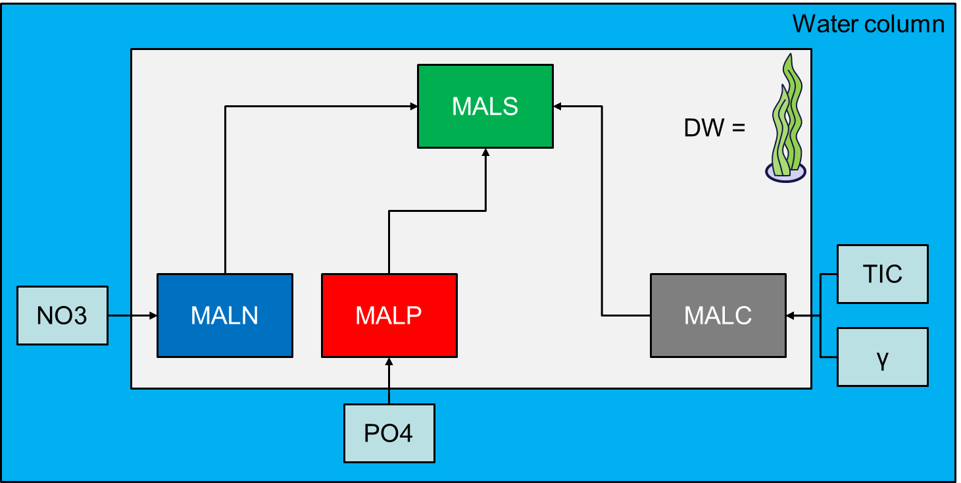
\includegraphics[width=1\linewidth]{figures/state_variables}
	\caption{Relationship between the state variables in MALG}
	\label{fig:statevariables}
\end{figure}
\textbf{MALS}: The structural mass represents the part of the macroalgae that increases the area and length of the total front when it grows. The surface area of the structural mass is the surface area available to capture solar energy. Structural mass does not take nutrients from the water, does not photosynthesize, and produces detritus when it decays/erodes. It grows by taking nutrients (N/P/C) from its storage exclusively and has its own fixed carbon, nitrogen, and phosphorous ratios that it must satisfy to grow. The structural mass has units of dry matter (gDM m$^{-2}$) and is similar to the common notion of 'dry matter'. However, it is less than the true dry matter content of the frond as measured using conventional methods because it represents only the dry weight of the plant minus the weight of water, nutrient stores, and carbon stores. The model also computes dry weight (DW) in the classical sense, which is the structural weight including the mass of nutrient stores, and wet weight (WW), which is the structural weight including the mass of nutrient stores and water. Both of these weights are model outputs and not state variables, although the units of structual mass are still described as grams of dry matter.
 
\textbf{MALN, MALP}: The nitrogen and phosphorous storage (or reserves) uptake dissolved inorganic nutrients (NH$_{4}^{+}$, NO$_{3}^{-}$, PO$_{4}^{3-}$) from the water column and store them for use by the structural mass during growth periods. In this model it is assumed the phosphorous storage dynamics are analagous to the nitrogen storage dynamics, but in reality the behaviour of phosphorous storage is not well known. Thus, phosphorous dynamics are coded but all fluxes and limitations are inactivated for the time being. Both NH$_{4}^{+}$ and NO$_{3}^{-}$ can be utilized based on a user-defined preference.

\textbf{MALC}: The carbon storage is the part of the plant responsible for photosynthesizing, producing exudate, and respiring. It produces carbon stores (carbohydrates) by taking up dissolved inorganic carbon and producing oxygen via photosynthesis. It provides carbon (energy) to the structural mass during growth periods. 

It is assumed that there is constant relationship between volume and area of a macroalgae frond. This means that the density of the macroalgae does not change, even if the ratio of structural mass to stored material changes. Additionally, the C:N and C:P ratios of each component are fixed, but because the ratio of stored mass to structural mass changes, the C:N and C:P ratios of the entire frond, and thus the dry matter, will change due to changes in the environment.
\pagebreak

\chapter{Overview of model subroutines}
\section{Distribution of macroalgae biomass in the water column}
\begin{flushright}
	\textsc{process: MALDIS}
\end{flushright}
The physiological equations described in \cite{broch2012} do not mention any physical description of the seaweed fronds in space aside from their area. In fact, area (m$^{2}$) is the state variable for structural mass in the Broch model. In spite of this fundamental difference it was found that the translation from an area based model to a DELWAQ mass based was possible. This is primarily because Broch uses a constant conversion factor between area and mass (called $ArDenMAL$ in MALG), and employs this factor in many of the model equations where mass rates concerning the structual mass are involved. Therefore, application of Broch's area based equations to DELWAQ's mass based system requires a fixed mass to surface area frond ratio and a DELWAQ segment surface area. In most cases the equations involving $MALS$ in MALG are simply \textit{not} multiplied by $ArDenMAL$ as the units are already in mass and not area. The largest implications of the difference between Broch and MALG relate to photosynthesis, which is proportional to the frond area and not the biomass. For these calculations, the $MALS$ mass is multiplied by the segment surface area and divided by the $ArDenMAL$ to obtain the frond area in the segment. For fluxes, a conversion is made to obtain the units of g m$^{-2}$ or g m$^{-3}$.  

Implementation in DELWAQ also requires knowledge of the vertical space occupied by the frond, which is not given by Broch. Thus, the algorithms for distributing the frond mass in space have been developed independently of the formulations in Broch. A simple approach is taken, whereby fronds (typically) only grow in length and retain a constant length:area ratio. The exception to this rule is when a frond is able to reach the end of the water column (i.e. the bed or the water surface) while it still has the capacity to grow. In these situations only the area will increase and not the length. The case for a single frond per computational cell is simple. However, MALG must be able to deal with any seeding density, which cannot be uniquely defined in a 3D model by the mass per m$^{2}$ in DELWAQ alone. For example, consider two cases whereby there exists 40g of dry matter per m$^{2}$ as is shown in Figure ~\ref{fig:ambiguoussituation}. 
\begin{figure}[H]
	\centering
	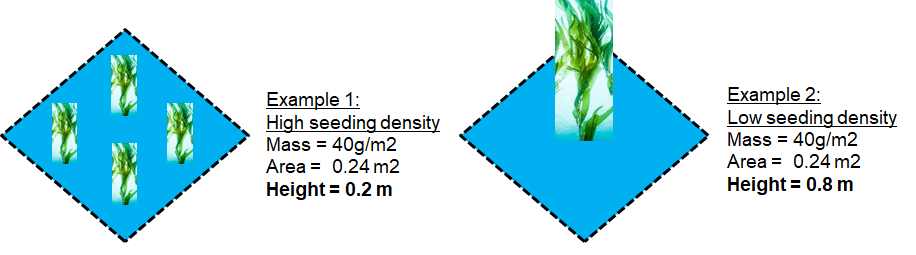
\includegraphics[width=1\linewidth]{figures/ambiguous_situation}
	\caption{Two situations that have identical mass but non-identical position of the mass in the vertical axis}
	\label{fig:ambiguoussituation}
\end{figure}
In the first example there are 4 fronds in a 1 m$^{2}$ square. They each weigh 10 g, have a combined area of 0.24 m$^{2}$ and are each 0.2 m long. In a second example, there is a single frond in a 1 m$^{2}$ square. It weighs 40 g, has an area of 0.24 m$^{2}$, and is 0.8 m long. In a 3D model with grid cells that are \textless 0.8 m thick, the nutrient uptake will take place in different cells in each of the two cases even though the mass per m$^{2}$ is identical in DELWAQ. To avoid this ambiguity the user must prescribe a set of parameters to describe the spatial characteristics of the culture. These are as follows:
\begin{itemize}
\item $FootDepth$ The depth below the water surface that the foot of the frond is attached. The frond begins growing from the segment that intersects this depth. The segment that the foot resides in can change with a variable water level because it is re-assigned each time step.
\item $LmaxMAL$ The maximum length of the frond measured in the vertical (z) axis from the foot to the tip of the frond. The frond cannot be longer than this value.
\item $SwGroMAL$ Switch for an upwards ($SwGroMAL$ \textgreater 0) or downwards ($SwGroMAL$ \textless 0) growing frond.
\item $LinDenMal$ The linear density of the culture. This describes the amount of mass it takes a single frond in 1 m$^{2}$ of culture to grow 1 m. All fronds in a single segment change length at the same rate as they grow.
\item $ArDenMal$ The area density of the culture. This is the ratio between surface area and dry weight.
\end{itemize}

The model does not explicitly model individual plants in a given segment, and so the collective mass per segment is generally referred to as a \textit{culture} in this model. Using the parameters described above, the culture's position can be completely described in 3 dimensions. To determine the position of the frond in the water column each time step, the process first calculates the length and the area of the culture in this column of segments:
\begin{equation}
\begin{aligned}
	&IF LinDenCor > 0\\
	&	LinDenFact = max(0.15 * (1 - (MALS/18.0)), 0.0)\\
	&ELSE\\
	&	LinDenFact = 0.0\\
	&END\\
	&LenMAL = min(F_{stretch} \times(LinDenFact + \frac{MALS}{LinDenMAL}), abs(LmaxMAL))\\
\end{aligned}
\end{equation}
\begin{equation}
	AreMAL = MALS \times \frac{Surf}{ArDenMAL}
\end{equation}


Where:\\

\begin{tabular}{ll}
$LenMAL$ & Length of culture in the column (m)\\
$Surf$ & Surface area of the bottom segment (m$^{2}$)\\
$MALS$ & structural mass (gDM m$^{-2}$)\\
$LinDenMAL$ & The linear density of a single frond (g m$^{-3}$)\\
$LinDenCor$ & 0 = do not correct the frond length, 1 = correct the frond length $(-)$\\
$LinDenFact$ & Frond length correction factor for low biomass density (in code only) $(-)$\\
$F_{stretch}$ & Factor by which to artificially make the frond longer and skinnier $(-)$\\

$ArDenMAL$ & The area density of the culture (g m$^{-2}$)\\
\end{tabular}

One of the central assumptions of a numerical model is that the system is homogeneous within a grid cell. Considering this, it is not meaningful to think of anything other than an equal distribution of fronds across each m$^{2}$ of the grid cell. When this distribution causes biomass densities to be extremely low (perhaps due to large grid sizes compared to the size of the farm), a very low biomass density multiplied by $LinDenMAL$ will yield a very short plant. The exchange with the ambient water will be correct but the vertical discretization will not be. 

To correct for this, the parameter $LinDenCor$ can be specified as = 1 to make the frond skinnier in order to have its length deviate from what would otherwise be calculated based on the mass per m$^2$. Setting $LinDenCor$ = 1 will make the culture possess the length of a normal individual frond without changing the biomass. A value of $LinDenCor$ = 0 will assign a length in accordance with the biomass present in the cell and no correction will be applied (this is the default setting). The correction factor is recommended for situations where the number of fronds per m${2}$ would be \textless\textless 1 (for more information on how the model deals with the number of fronds, see subroutine FLMALS.f). This intercept $LinDenFact \times F_{stretch}$ is determined by the initial biomass condition and is only calculated at the beginning of the simulation and does not change. To further adjust this length beyond correcting for biomass density, I.e. to incorporate the effect of ropes, you can adjust the factor $FrondStrech$. This will simply multiply the computed length by a constant to elongate the frond and spread the biomass and the fluxes over more segments.

$LenMAL$ is then used to check which segments the frond biomass should be present in, and which fraction of the frond exists in each segment. This fraction is communicated to each segment for all other computations involving biomass and fluxes. As all MALG parameters are non-transportable (g m$^{-2}$), by DELWAQ convention only the bottom segment can technically contain any MALG mass. However, depending on the ratio of segment depths to frond length, the culture can exhibit fluxes affecting segments other than the bottom segment. To achieve this effect without actually storing any mass in segments above the bottom segment, MALDIS tells each segment what fraction of the biomass in the water column resides in any particular segment ($FrBmLay$), and also the mass of this biomass as the parameter $BmLayMAL$. Still, all mass actually administratively resides in the bottom segment.

The calculation of this biomass fraction depends firstly on whether the frond grows upwards or downwards.

\begin{equation}
Zm =  
\left 
.\begin{tabular}{cc}
$SwGroDir < 0:$& $LenMAL + FootDepth$\\
$SwGroDir > 0:$& $FootDepth - LenMAL$\\
\end{tabular}
\right
.\end{equation}

Where:\\

\begin{tabular}{ll}
$Zm$ & Distance from water surface to tip of frond (positive down) (m)\\
$Z1$ & Distance from water surface to top of segment (positive down) (m)\\
$Z2$ & Distance from water surface to bottom of segment (positive down) (m)\\
\end{tabular}

The segment top depth $Z1$ and segment bottom depth $Z2$ are then checked against $Zm$ to see if the frond resides entirely within, entirely outside, or partially within the current segment in the segment loop. The fraction of the biomass allocated to the current segment is then the ratio of the segment depth to $LenMAL$ in the column for segments in which the frond completely resides, or the ratio of the difference between $Zm$ and either $Z1$ or $Z2$ to $LenMAL$ for segments in which the tip or foot of the frond is found.

Experiments done by \cite{sjotun1993} show that the length of \textit{Saccharina} can vary between 0.8 m and 1.6 m, and the growth in length of the fronds varied between 0.1 and 1.2 cm d${^-1}$. The length to width ratios of the new frond material varied quite a bit, but during periods of high growth it was approximately 0.5. Thus, it is assumed that for every cm gained in length there are 2 cm gained in width. Note that the overall shape of the plant is such that the L/W ratio is \textgreater 1, because it is only new material that grows at a ratio less than 1. Taking the \cite{broch2012} value of 0.6 g sw dm${^-2}$ (60 g) as the area density, it is found that the plant is expected to require 0.003 g sw cm$^{-1}$ of growth in length. Thus, the default value for $LinDenMAL$ is set to 0.3 g sw m$^{-1}$.

\pagebreak

\section{Flux of Macroalgae structural biomass}
\begin{flushright}
\textsc{process: FLMALS}
\end{flushright}

The structural component of the macroalgae is the dry material that gives shape and structure to the macroalgae frond. It does not include N, P, or C stores, but has a fixed N, P, and C component. This means that these nutrients are required for growth of the structural mass, and that there is a minimum amount of N,P and C in the structural mass regardless of the reserve nutrient level. As the structural mass grows it increases the length and area of the entire frond. Growth of other components of the frond (nutrient reserves) do not have any effect on the frond length, volume, density, or surface area. 

The net growth of the structural mass is the resulting rate of structural biomass production and frond erosion (considered to be analagous to mortality used in other DELWAQ processes). This balance can be defined by the following equation:
\begin{equation}
	dGrowMALS =MALS \times (\mu - \phi)
\end{equation}

Where:\\
\begin{tabular}{cc}
	$\mu$  & specific growth rate of macroalgae sturctural mass (d$^{-1}$) \\
	$\phi$ & mortality/erosion rate (d$^{-1}$) \\
\end{tabular}

The growth rate $\mu$ of $MALS$ is dependent firstly on the available nutrient stores ($MALN$, $MALP$, and $MALC$). The growth rate is defined as follows:
\begin{equation}
	\mu = f_{density} f_{photoperiod} f_{temperature}\times min\big\{1-\frac{N_{min}}{MALN},1-\frac{P_{min}}{MALP},1-\frac{C_{min}}{MALC}\big\}
\end{equation}

Where:\\

\begin{tabular}{ll}
$f_{density}$ & biomass density limitation function (-)\\
$f_{photoperiod}$ & photoperiod limitation function (-)\\
$f_{temperature}$ & temperature limitation function (-)\\
$N_{min}$ & minimum N storage (gN gDM$^{-1}$)\\
$MALN$ & nitrogen storage (gN/m$^2$)\\
$P_{min}$ & minimum phosphorous storage (gP gDM$^{-1}$)\\
$MALP$ & phosphorous storage (gP/m$^2$)\\
$C_{min}$ & minimum carbon storage (gC gDM$^{-1}$)\\
$MALC$ & carbon storage (gC/m$^2$)\\
\end{tabular}

Note that in the code the storage terms are temporarily converted from $gX m{^-2}$ to $gX/gDM_{structural}$ by dividing by $MALS$ to comply with the formulations and units outlined in \cite{broch2012} where they have units of $gX/gDM_{structural}$. In MALG formulations, the storage state variable terms are (must be) g m$^{-2}$ as per all non-transportable DELWAQ substances. This is reflected in the fluxes, which are back calculated to g m$^{-2}d^{-1}$. As the substances are non transportable, they reside in the bottom segment. However, depending on the user defined variables, it is possible for the mass and associated fluxes to have no effect in the bottom segment, such as in the case where the algae grow from the water surface downward. This is discussed in MALDIS.

$gDM_{structural}$ is not equivalent to dry matter, and it does not include the nutrient stores. The outputs dry weight and wet weight are calculated by the model according to the following equations:
\begin{equation}
\begin{aligned}
&Wdry = MALS(1 + k_N(MALN - (MALN_{min})) + \\
&MALN_{min} + k_C(MALC - MALC_{min})+ MALC_{min})
\end{aligned}
\end{equation}

\begin{equation}
\begin{aligned}
&Wwet = MALS(\frac{1}{k_D} + k_N(MALN - (MALN_{min})) + \\
&MALN_{min} + k_C(MALC - MALC_{min}) + MALC_{min})
\end{aligned}
\end{equation}

Where:\\
\begin{tabular}{ll}
$k_C$        & carbon:dry matter ratio in structural mass (gC gDM$^{-1}$)\\
$k_N$        & nitrogen:carbon ratio in structural mass (gN gC$^{-1}$)\\
$k_W$        & dry weight to wet weight ratio in structural mass (g g$^{-1}$)\\
\end{tabular}
The growth rate of the structural mass is dependent on a density limitation, a photoperiod limitation, and a temperature limitation. These limitations differ from conventional DELWAQ limitations for algae growth in that they do not range strictly between 0 and 1 and alter a pre-defined growth rate. Instead, Broch has tuned them such that their product is equal to the maximum growth rate when conditions are optimal (0.18 d$^{-1}$). 

The density limitation represents the ability of the frond to only grow so big, and the bigger it gets the lower its growth rate will become. The formulation is as follows:
\begin{equation}
f_{density} = m_1 exp\big\{-(\frac{SpecArea}{MALS_0})^2 \big\}+m_2
\end{equation}

Where:\\

\begin{tabular}{ll}
	$m_1$    & growth rate parameter 1 (-)\\
	$m_2$    & growth rate parameter 2 (-)\\
	$SpecArea$ & Specific area per frond (m$^2$)\\
	$MALS_0$ & critical biomass area (m$^2$)\\
\end{tabular}

$SpecArea$ is defined as follows:\\

\begin{equation}
NFrond = \frac{DryWeight \times Surf}{SeedMass}
\end{equation}
\begin{equation}
SpecArea = \frac{TotAreMAL}{NFrond} 
\end{equation}

Where:\\

\begin{tabular}{ll}
	$NFrond$ & Number of fronds in segment\\
	$TotAreMAL$    & Total area of culture in column (m$^2$)\\
	$SeedMass$ & mass in DW of a frond at seeding (gDW)\\
\end{tabular}

This formulation is designed to allow small fronds to grow faster than bigger fronds, and as such the $MALS_0$ value in Broch describes the area above which a frond will stuggle to grow well. This has large implications for the DELWAQ model, as the Broch model is 'individual based' rather than 'culture based'. DELWAQ does not \textit{a priori} know nor does it explicitly model how many fronds there are in a segment, only the mass and area of the culture. However, it must know how big any given frond is to determine the rate at which the culture erodes and is limited by density. Thus the size must be known independently of the segment geometry. With the assumption that mass is equally distributed across any model segment, the height and area per m$^2$ resulting from a uniform distribution of mass can be incredibly small when the farm size is much smaller than the segment size. To calculate a sensible representative frond area to determine the density limitation, the parameter $SpecArea$ is defined to represent the area of a single frond, of which there are $NFrond$ of per segment. This $NFrond$ number is calculated in the first time step and is derived from the sum of all frond areas in a segment and a parameter called $SeedMass$. This seed mass must be specified by the user and represents the mass of an individual seed at the time of seeding. Note that $NFrond$ is only stored in the bottom segment and describes the number of fronds in the column.

The photoperiod limitation is similar to the daylength limitation used in BLOOM and DYNAMO, but instead considers the \textit{normalized change} in daylength compared to the previous day instead of the actual current daylength. In this context, 'normalized' means that the change in daylength is relative to the maximum change in daylength (i.e. the daylength change at the equinoxes). This response to normalized daylength change is due to the fact that \textit{Saccharina latissima} is a seasonal anticipator and will grow and store nutrients in accordance with the change in the season as determined by how much longer or shorter the days become. This formulation is given by: 
\begin{equation}
f_{photoperiod} = a_1 (1+sin(\tau (n) | \tau (n)| ^{\frac{1}{2}})) + a_2
\end{equation}

Where:\\

\begin{tabular}{ll}
	$a_1$    & photoperiod parameter 1 (-)\\
	$a_2$    & photoperiod parameter 2 (-)\\
\end{tabular}

and $\tau$ is a function describing the normalized difference in day length between current day and previous day. This function is calculated by the process DAYLP which essentially identical to the standard DELWAQ process DAYL. The parameters $a_1$ and $a_2$ are chosen such that $0.3 \textgreater f_{photoperiod} \textless 2$ at the given latitude. In future implementations it is hoped that the code will calculate this for the user, but it currently requires an iterative approach before the simulation to define the correct values for the given latitude to  ensure $0.3 \textgreater f_{photoperiod} \textless 2$.

The temperature limitation is a simple piece wise function that identifies an optimal growth between temperatures 10-15$^0$C, no growth above 19$^0$C, and linear growth increasing between -1.8 and 10$^0$C. The temperature limitation is therefore:
\begin{equation}
f_{temperature} =  
\left 
.\begin{tabular}{cc}
$ 0.08T + 0.2 $    & $-1.8 \textless 10$ \\
$  1 $             & $10 \leq T \leq 15$ \\
$19/4 - T/4$       & $15 \leq T \leq 19$ \\ 
$0$                & $T \textgreater 19$ \\
\end{tabular}
\right
.\end{equation}

The specific erosion (mortality) rate $\phi$ of the structural biomass is proportional to the area of the frond and the erosion parameter. The formulation is as follows:
\begin{equation}
\phi = \frac{10^{-6}exp(\epsilon\times SpecArea)}{1+10^{-6}exp((\epsilon\times \frac{LocArea}{N_{frond}})-1)}
\end{equation}

Where:\\
\begin{tabular}{ll}
$\epsilon$ & erosion parameter (m$^{-2}$)\\

\end{tabular}

Here it can be seen that using the same logic described for the implementation of the density limitation, the mortality rate is adjusted to account for the true area of a single frond ($SpecArea$) regardless of seeding density in the segment. This correction is in place to account for the fact that the dimensions of the representative frond in the culture determines the mortality (and density limitation) of the culture.

The structural growth process occurs over all segments which have a biomass fraction \textgreater 0. This is in spite of the fact that the biomass administratively resides in the bottom segment. During each time step, all segments with a non-zero biomass fraction receive 'ghost' structural and storage mass according to the biomass allocated to it in MALDIS. The local inorganic nutrient, gas, and particulate fluxes are calculated using this mass and the local ambient conditions. The fluxes are then locally applied to ambient state variables exogenous to MALG, but not the MALG parameters ($MALS$, $MALN$, $MALP$, $MALC$). Instead, the fluxes of MALG state variables are communicated to the bottom segment in a cumulative way, whereby the local fluxes of all segments that share the same bottom segment are summed to compute the net total change in $MALS$, $MALN$, $MALP$, and $MALC$ resulting from the net growth in the column. 

Once the bottom segment is reached in the segment loop, the fluxes for each column of segments have been accumulated and the net change in mass of each administrative bottom segment is known. The culture will then become longer or shorter in the next time step to reflect this new state, which again is kept track of by the bottom segment in the column. The consequence of applying this technique is that the local per segment 'ghost reserve masses' adopt the reserve ratio of the whole column. Another way to say this is that all segments with a non-zero biomass fraction belonging to a given water column have a fixed structural mass to storage mass ratio, and consequently all reserves are equally distributed along the frond.
\pagebreak

\section{Flux of Macroalgae nutrient storage}
\begin{flushright}
\textsc{process: FLMALN}
\end{flushright}

The nutrient storage component(s) of the macroalgae (also referred to as reserves) are those that supply nutrients for growth of the structural mass. The storage is also responsible for taking up dissolved inorganic nutrients from the ambient water. The reserves consist of a nitrogen ($MALN$) and a phosphorous ($MALP$) storage component, which are both dealt with in the same nutrient storage subroutine. Note that \cite{broch2012} does not include a phosphorous component to the nutrient storage, but it is included in this model for flexibility should new information about phosphorous storage become available. Currently the model is written such that the culture cannot be P limited and no P flux will occur.

The change in a nutrient storage mass is given by the following equations:
\begin{equation}
dUptMALN = J_N - \mu(k_C \times k_N \times MALS + MALN)
\end{equation}
\begin{equation}
dUptMALP = J_P - \mu(k_C \times k_P \times MALS + MALP)
\end{equation}

Where the state variables $MALN$ and $MALP$ are in the units given by Broch (gX/gDM), which is achieved in MALG by dividing $MALX$ by $MALS$ at the begining of the subroutine. This is valid because the storage is distributed equally along the frond. This equation represents the balance between uptake $J$ and utilization for growth of the frond's structural mass $\mu$. The uptake is dependent on flow velocity, the amount of stores compared to the minimum and maximum possible, and the ambient nutrient concentration. The formulation for both nitrogen and phosphorus is described as follows:
\begin{equation}
J_N = f_{velocity}J_{Nmax}(\frac{NO_3^-}{K_{sn}+NO_3^-})(\frac{MALN_{max}-MALN}{MALN_{max}-MALN_{min}})
\end{equation}
\begin{equation}
J_P = f_{velocity}J_{Pmax}(\frac{PO_4^{3-}}{K_{sp}+PO_4^{3-}})(\frac{MALP_{max}-MALP}{MALP_{max}-MALP_{min}})
\end{equation}
\begin{equation}
f_{velocity} = 1-exp(-\frac{U}{U_{0.65}})
\end{equation}

Where:\\

\begin{tabular}{ll}
$k_P$        & phosphorous:carbon ratio in structural mass (gN gC$^{-1}$)\\
$J_{Nmax}$   & maximum uptake rate nitrogen (gN m$^{-2}$d$^{-1}$)\\
$K_{sn}$     & half saturation for inorganic nitrogen uptake\\
$NO_3^-$     & ambient nitrate concentration (gN m$^{-3}$)\\
$MALN_{max}$ & maximum nitrogen storage (gN gDM$^{-1}$)\\
$MALN_{min}$ & minimum nitrogen storage (gN gDM$^{-1}$)\\
$J_{Pmax}$   & maximum uptake rate nitrogen gP m$^{-2}$d$^{-1}$)\\
$K_{sp}$     & half saturation for inorganic nitrogen uptake (gP m$^{-3}$)\\
$PO_4^{3-}$  & ambient phosphate concentration (gP m$^{-3}$)\\
$MALP_{max}$ & maximum phosphorous storage (gP gDM$^{-1}$)\\
$MALN_{min}$ & minimum phosphorous storage (gP gDM$^{-1}$)\\
$U$          & water velocity (m s$^{-1}$)\\
$U_{0.65}$   & water velocity at which uptake rate is 65 of maximum (m s$^{-1}$)\\
\end{tabular}

The first term in $J_{N}$ and $J_{P}$ pertains to the uptake of nutrients and the second term to the utilization of stores by the structural mass during growth. Note how the nutrient requirement (quota) is dependent on the combined quota for structural mass and storage mass. The uptake of nutrients is dependent on the ambient concentration according to Michaelis-Menten kinetics. It is dependent on velocity such that high velocities make it easier for the frond to uptake the nutrients. This is related to an improved mass transfer coefficient. At sufficiently high ambient concentrations and water velocities the uptake rate is $J_{max}$.
\pagebreak

\section{Flux of Macroalgae carbon storage}
\begin{flushright}
\textsc{process: FLMALC}
\end{flushright}

The carbon storage component of the macroalgae ($MALC$) supplies carbohydrates for growth of the structural mass. The carbon storage is also responsible for photosynthesis, respiration and exudation. The change in a carbon storage mass is given by the following equation:
\begin{equation}
dUptMALC = P(1-E)-R - \mu(k_C \times MALS + MALC)
\end{equation}

Where:\\

\begin{tabular}{ll}
$P$ & Gross photosynthetic rate (gCm$^{-2}$ d$^{-1}$)\\
$E$ & Fraction exudation (-)\\\
$R$ & Maintenance respiration rate (gCm$^{-2}$ d$^{-1}$)\\
\end{tabular}

Where the first term relates to the net of production, respiration and exudation, and the second term pertains to the utilization of carbon stores by the structural mass. The state variable $MALC$ is given here in the units used by Broch (gC/gDM), which is achieved in MALG by dividing $MALC$ by $MALS$ at the begining of the subroutine. This is valid because of the assumption that the storage is distributed equally along the frond.

The carbon production rate (i.e. photosynthesis) as a function of temperature ($T$) and irradiance ($I$) is given by the following set of equations:
\begin{equation}
P(T,I) = P_s(1-exp(-\frac{\alpha \times I}{P_s}))exp(-\frac{\beta \times I}{P_s})
\end{equation}
\begin{equation}
P_s(T) = \frac{\alpha \times I_{sat}}{ln(1+\frac{\alpha}{\beta})}
\end{equation}
\begin{equation}
P_{max}(\beta) = (\frac{\alpha \times I_{sat}}{ln(1+\frac{\alpha}{\beta}})(\frac{\alpha}{\alpha+\beta})(\frac{\beta}{\alpha+\beta})^{\frac{\beta}{\alpha}}
\end{equation}
\begin{equation}
P_{max}(T) = \frac{P_1exp(\frac{T_{AP}}{T_{P1}})}{1+exp(\frac{T_{APL}}{T} - \frac{T_{APL}}{T_{PL}})+exp(\frac{T_{APH}}{T_{PH}}-\frac{T_{APH}}{T})}
\end{equation}

Where:\\

\begin{tabular}{ll}
$P$ & Photosynthetic rate (gC dm$^{-2}$ h$^{-1}$)\\
$P_s(T)$ & Saturation photosynthetic rate (gC dm$^{-2}$ h$^{-1}$)\\
$I$ & Incident radiation (W m$^{-2}$)\\
$I_{sat}$ & Saturation radiation (W m$^{-2}$)\\
$\alpha$ & Photosynthetic efficiency (gC dm$^{-2}$ h$^{-1}$ ($\mu$mol$_{p}$ m$^{-2}$ s$^{-1}$)$^{-1}$) \\
$\beta(T)$ & Photosynthetic light inhibition (gC dm$^{-2}$ h$^{-1}$ ($\mu$mol$_{p}$ m$^{-2}$ s$^{-1}$)$^{-1}$) \\
$P_1$ & Reference photosynthetic rate at T$_1$ ($^{0}$K)\\
$P_2$ & Reference photosynthetic rate at T$_2$ ($^{0}$K)\\
$T$ & Water temperature ($^{0}$K)\\
$T_{P1}$ & temp for reference photosynthetic rate 1 ($^{0}$K)\\
$T_{P2}$ & temp for reference photosynthetic rate 2	($^{0}$K)\\
$T_{AP}$ & Arrhenius temperature for photosynthesis ($^{0}$K)\\
$T_{APH}$ & Arrhenius temp for photosynthesis high end ($^{0}$K)\\
$T_{APL}$ & Arrhenius temp for photosynthesis low end ($^{0}$K)\\
\end{tabular}

Note the use of unconventional DELWAQ units dm$^{2}$, $\mu$mol (photons), and hours. These have been maintained to allow easy comparisons to Broch and to emphasize the fact that photosynthesis is proportional to frond \textit{surface area} and not segment surface area in MALG. There is an internal conversion in the code from $W$, the unit of DELWAQ radiation, to $\mu$mol s$^{-1}$, the unit of irradiance in the formulations, which is 4.57 $\frac{\mu mol s^{-1}}{W}$. After production, respiration and exudation have been calculated, all rates are converted to gC m$^{-2}$ d$^{-1}$ by multiplying by 2400. Recall that this is still in m${^2}$ of frond per segment, and so this is further multiplied by the total area of frond in the segment, which is later divided by the segment surface area to get the gross production flux.

It would be possible for this routine to receive information about the light environment in the water column from the process $CALCRAD$. However, the first implementation of the MALG module was meant to be independent of other DELWAQ processes. For integration into DELWAQ, the previous day length and the light environment should be provided to MALG processes instead of being calculated by MALG processes. Currently, irradiance in MALG is calculated using the same equations as is used in DYNAMO, using the surface irradiance, the extinction of visible light, and the water depth, while integrating the Lambert-Beer equation over the current segment using the following equation:

\begin{equation}
I = \frac{-I_{0}e^{-ExtVl \times LocalDepth}}{ExtVl \times Depth}  - e^{-ExtVl \times (LocalDepth - Depth)}
\end{equation}

Where:\\
\begin{tabular}{ll}
$I_{0}$ & Irradiance at the surface (W m$^{-2}$)\\
$ExtVl$ & Extinction of visible light (m$^{-1})$\\
$Depth$ & Thickness of segment (m)\\
$LocalDepth$ & Depth of bottom of segment below water surface (m)\\
\end{tabular}

Currently the macroalgae do not contribute to light attenuation in the water column.

This set of equations describes a photo inhibitory effect for $I\textgreater I_{sat}$. The structural mass is strictly unable to grow above $T \textgreater 19^{0}$. Although the structural mass cannot grow, photosynthesis production can still occur in the range -1$^{0}$C $\textgreater T \textless$ 23$^{0}C$. These two temperature controls are fixed for the species and the user cannot flexibly change this unless the code is edited. To adapt the model to tropical species or species that have a different optimal temperature photosynthesis range, both the temperature function and the photosynthetic range parameters have to be edited in addition to the code for the piece-wise temperature growth function for $MALS$.

The formulations also show that the maximum production rate $P_{max}$ can be expressed in two ways. The first is only a function of temperature and describes photosynthesis at $I = I_{sat}$. The second production rate $P_{max}$ is the actual maximum production rate taking into account the effect of temperature on the response of growth to light. This means that growth is non-linear in temperature, as it effects both growth directly and also the way in which growth is affected by light. $\beta$ is solved for using Newton's method in Broch by differentiating $P_{max}(\beta)$. This involves solving for the value $\beta$ such that $P_{max}(T)$ equals the $P_{max}(\beta)$ obtained from the temperature relationship at the current temperature and at $I = I_{sat}$. Newton's method is not used in the DELWAQ code and instead $\beta$ is pre-calculated for all temperatures in the photosynthetic range -2$^{0}$C to 23$^{0}$C at an interval of 0.1$^{0}$C. This is hard coded into the FLMALC subroutine and constitutes a linear approximation of $\beta$. Due to this the model should only be used for temperature ranges $-2^{0}C \textless T \textless 23^{0}C$. Currently:
\begin{itemize}
	\item $\beta(T)$ for $T \textless -2^{0}C = \beta(-2^{0}C)$ and $\beta(T) for T > 23^{0}C = \beta(23^{0}C)$. 
\end{itemize} 

Consequently, temperatures above or below the photosynthetic temperature range will result in a production rate equivalent to the rate at the closest temperature in the range. The relationship between temperature, beta, irradiance and gross production is shown in Figure ~\ref{fig:lightequations}

\begin{figure}[H]
	\centering
	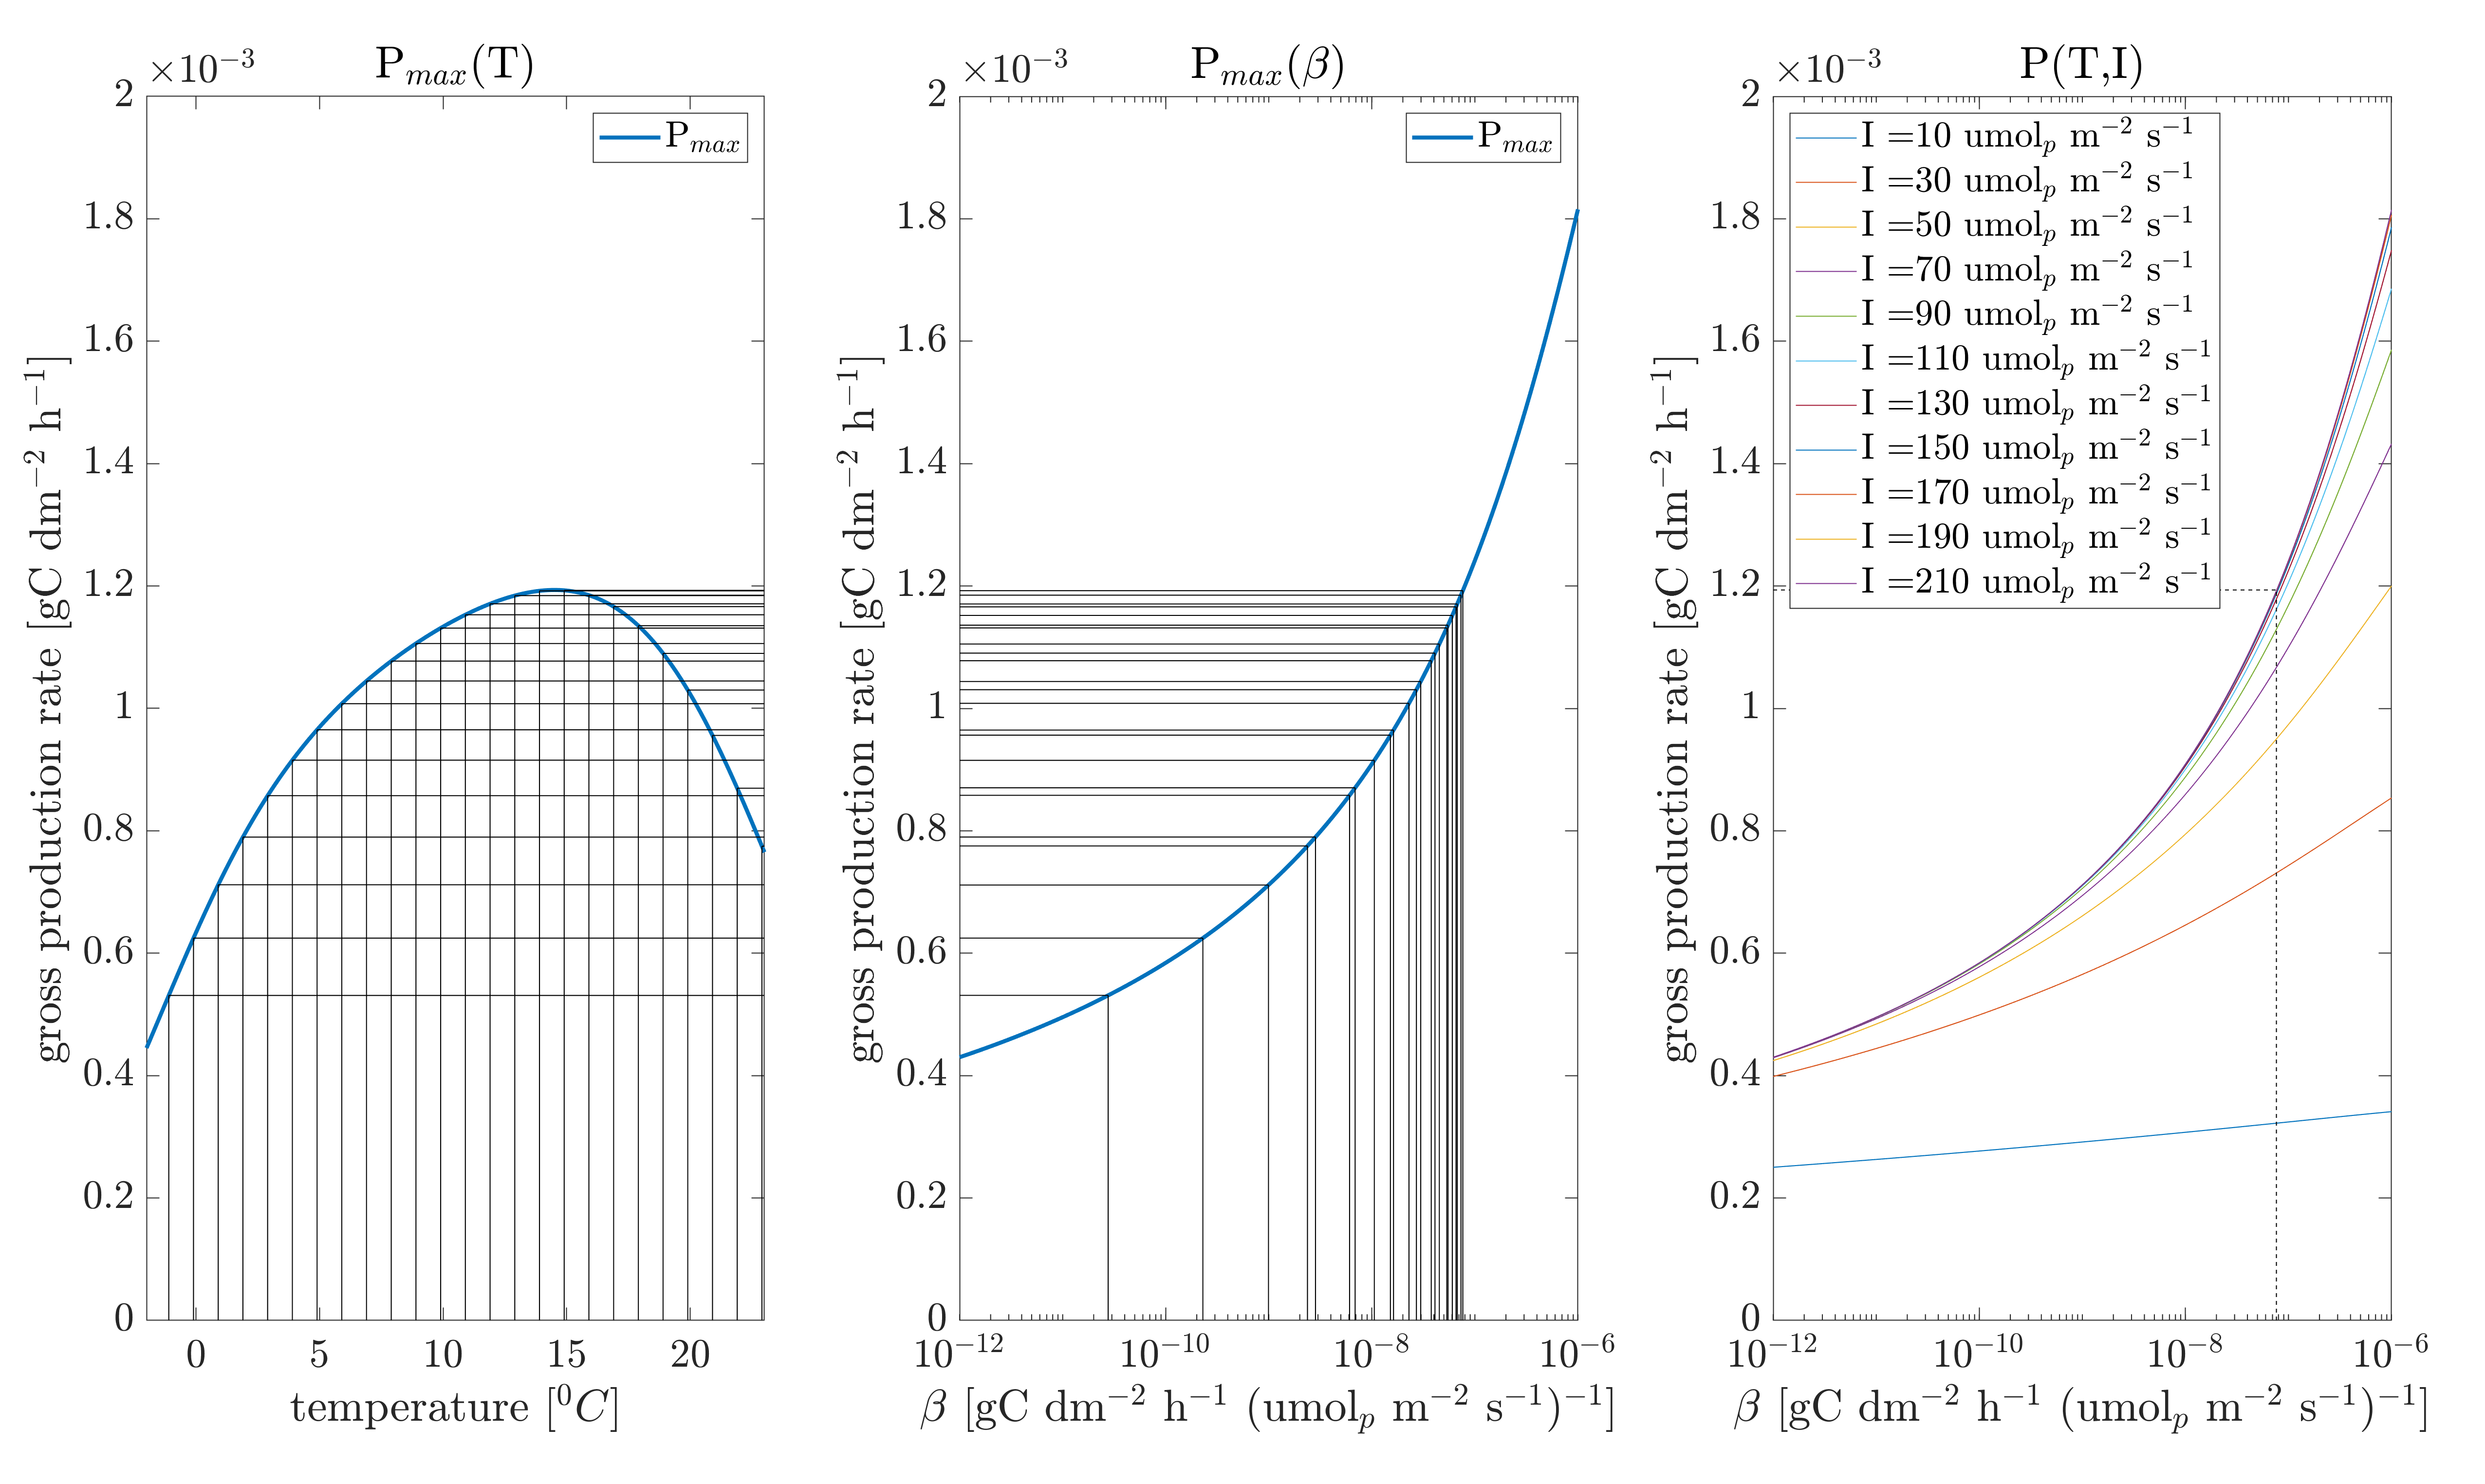
\includegraphics[width=1\linewidth]{figures/light_equations_crop}
	\caption[]{Relationship between temperature, $\beta$, irradiance and gross production. Here the black lines demonstrate the process by which for a given temperature $P_{max}(T)$ is calculated, and the corresponding $\beta$ value required to achieve $P_{max}(T) = P_{max}(\beta)$ is derived, and used to calculate the response of growth rate to irradiance, where $P = P_{max}$ when $I = I_{sat}$}
	\label{fig:lightequations}
\end{figure}
\pagebreak

\section{Harvesting of macroalgae}
\begin{flushright}
	\textsc{process: HRVMAL}
\end{flushright}
Seaweed act as bioremediators of the marine IMTA environment, but they are also a 'crop' that can be used as food or sources of pharmaceutical products. This means that they are also harvested periodically. This process of harvesting seaweed biomass is incorporated in MALG using a simple harvesting routine.
\begin{equation}
dHrvMALS = K0HrvMALS + MALS \times K1HrvMALS\\\
\end{equation}
\begin{equation}
dHrvMALN = dHrvMALS \times \frac{MALN}{MALS}\\
\end{equation}
\begin{equation}
dHrvMALP = dHrvMALS \times \frac{MALP}{MALS}\\
\end{equation}
\begin{equation}
dHrvMALC = dHrvMALS \times \frac{MALC}{MALS}\\
\end{equation}

Where:\\

\begin{tabular}{ll}
	$K0HrvMALS$ & Zero-order harvesting rate of MALG (g DM m$^{-2}$ $d{^-1}$)\\
	$K1HrvMALS$ & First-order harvesting rate of MALG ($d{^-1}$)\\
\end{tabular}

$dHrvMALS$ is set to = 0 if $MALS < dHrvMALS\times \delta t$
 
\pagebreak

\chapter{Usage tips}
\section{A note about model output in MALG}
This module is somewhat different from other DELWAQ modules because of the notion of ghost mass. This means that although it follows DELWAQ convention that state variables are written to the bottom segment (where they administratively reside), outputs like gross production are written to segments that the ghost mass resides in. This means that the user must be aware of what is written to which segments. There are some values that are (1) only written to the bottom layer, (2) written to individual segments only if the segments have ghost biomass, and (3) written to all segments in a water column that have some biomass in the bottom layer. The clarification of which is which is now described using definitions congruent with the proces.asc file:

\textbf{Type 1.} State variables strictly always exist only in bottom segments:
\begin{itemize}
	\item MALS     : MacroALgae Structural biomass                          (gDM/m2)        
	\item MALN     : MacroALgae Nitrogen storage                            (gN/m2)       
	\item MALP     : MacroALgae Phosphrous storage                          (gP/m2)       
	\item MALC     : MacroALgae Carbon storage                              (gC/m2)  
\end{itemize}

\textbf{Type 2.} Outputs that reflect what is happening in the specific segment and is = 0 for segments without biomass, including bottom segment if FrBmLay == 0:
\begin{itemize}
	\item BmLayMAL : Biomass of MALS in segment                              (gDM/m3) 
	\item BrochP   : gross production as per Broch                           (gC/dm2/h) 
	\item ExudMALC : exudation MALC                                          (gC/m2/d)  
	\item FrBmMALS : Fraction of bottom layer MALS in this seg               (-)         
	\item GrosMALC : gross photosynthesis MALC                               (gC/m2/d)  
	\item LimDenS  : biomass density limitation MALS                         (-) 
	\item LimMALC  : carbon storage limitation MALS                          (-) 
	\item LimMALN  : nitrogen storage limitation MALS                        (-) 
	\item LimMALP  : phosphrous storage limitation MALS                      (-) 
	\item LimN     : ambient nitrogen limitation for storage                 (-) 
	\item LimNutS  : net nutrient storage limitation MALS                    (-) 
	\item LimP     : ambient phosphorous limitation for storage              (-) 
	\item LimPhoS  : photoperiod limitation MALS                             (-) 
	\item LimTemS  : temperature limitation MALS                             (-) 
	\item LimVel   : velocity limitation                                     (-) 
	\item LocDecS  : local decay of MALS                                     (DM/m2/d) 
	\item LocGroC  : local utilization of MALC by MALS                       (gC/m2/d) 
	\item LocGroN  : local utilization of MALN by MALS                       (gN/m2/d) 
	\item LocGroP  : local utilization of MALP by MALS                       (gP/m2/d) 
	\item LocGroPS : local gross production of MALS                          (DM/m2/d) 
	\item LocNetPS : local net production of MALS                            (DM/m2/d) 
	\item LocUpC   : Local C storage uptake flux in this segment             (gC/m2/d) 
	\item LocUpN   : Local N storage uptake flux in this segment             (gN/m2/d) 
	\item LocUpP   : Local P storage uptake flux in this segment             (gP/m2/d) 
	\item muMALS   : unit growth rate MALS                                   (1/d) 
	\item RespMALC : respiration MALC                                        (gC/m2/d)         
	\item WDry     : dry weight of culture in segment                        (g/m2) 
	\item Wwet     : dry weight of culture in segment                        (g/m2) 
	\item WdryTot  : dry weight of culture in segment                        (g) 
	\item WwetTot  : wet weight of culture in segment                        (g)  
\end{itemize}

\textbf{Type 3.} Outputs that reflect what is happening in the column, and all segments in the column have the same value:
\begin{itemize}
	\item MALCDMS   : macroalgae C storage in column w.r.t structural        (gC/gDM)
	\item MALNDMS   : macroalgae N storage in column w.r.t structural        (gN/gDM)
	\item MALPDMS   : macroalgae P storage in column w.r.t structural        (gP/gDM) 
	\item MALSCDM   : ratio C:DM in whole frond                               (gC/gDM) 
	\item MALSNDM   : ratio N:DM in whole frond                               (gN/gDM) 
	\item MALSPDM   : ratio P:DM in whole frond                               (gP/gDM) 
	\item MALSNC    : ratio N:C in whole frond                                (gN/gC) 
	\item MALSPC    : ratio P:C in whole frond                                (gP/gC) 	
	\item FootDepth : location of frond attachment in the water column < MSL (m)   
	\item FrondArea : area of each individual frond in segment               (m2/m2/frond)    
	\item LocAreaMAL: area of all fronds per m2 of column                    (m2/m2)          
	\item TotAreaMAL: area of frond in this column                           (m2) 
	\item LengthMAL : length of frond in this column                         (m)  
	\item TipDepth  : depth of tip of frond in this column                   (m)  
\end{itemize}

The python script /MALG/testbench/plot\_FARM.py contains a function that can extract information from the his file based on the rules stated above. It relies on the dictionary contained in /MALG/testbench/per\_Segment\_per\_Column.py.

\section{Initializing macrolalgae in a DELWAQ model}

The units in MALG are not the type that one expects to obtain from farm designs or measurements. Typically one might know how much mass there is at the beginning of the growing season, or how many sporophytes are seeded. The model however used mass per square meter, and internally translates this to Broch units (gX gSW ${-1}$). Using the following steps and equation 2.6 you can obtain a good initial condition for your model.\\
\begin{itemize}
	\item Probably the initial mass (gDW) of the seaweed is known.
	\item Divide this number by the surface area of the grid cell you are putting the seaweed in.
	\item Equation 2.6 describes the relationship between dry weight and structural weight. Use it to solve for MALS (gC m$^{-2}$) by choosing an initial condition for the broch parameters MALN (gN gSW$^{-1}$) and MALC (gC gSM$^{-1}$) that describe the stores of the algae. Recommended values are 0.01 gN gSW$^{-1}$ and 0.6 gC gSW$^{-1}$.
	\item Calculate MALN (gN m$^{-2}$) and MALC (gC m$^{-2}$) by multiplying the Broch MALN and MALC by MALS.
	\item Set $LinDenCor$, $F_{stretch}$, $SWGroDir$, $LmaxMAL$, and $SeedMass$ according to the situation.. 
	\item If using FStretch, you can calculate an appropriate value by multiplying the desired length of the culture by $\frac{1}{0.15}$. Using $F_{stretch}$ is recommended for mass densities \textless 18 gSW m$^{-2}$. 
	\item \textbf{Reminder}: Photoperiod parameters $a1$ and $a2$ must be chosen to satisfy $0.3 \textgreater f_{photoperiod} \textless 2$ at the desired latitude. This is not calculated automatically and must be provided by the user. One can use the python script /MALG/code/py/DAYLP.py to find optimal values for a1 and a2 given a latitude.
	\item \textbf{Reminder}: Temperature limitations are hard-coded in for Atlantic species that experience optimal growth between 10-15$^0$C.
\end{itemize}

\pagebreak

\chapter{Model validation}
This section briefly outlines the test cases for the application of the MALG model. Two test cases have been outlined:
\begin{itemize}
	\item Broch 1DV model
	\item A simple (large) 3D flume model with tidal currents
\end{itemize}
\section{Testcase: Broch 2012}
This testcase involves the reproduction of the model as it was demonstrated in \cite{broch2012}. The testcase in Broch involves a single frond growing off the coast of Nowrway in 250m deep water at approximately 5 m below the surface, although the depth of the frond in \cite{broch2012} is never explicitly stated. The kelp grows in a 0D model (a box) with temperature, nitrogen, and light climate forcing derived from measurements and local models. These forcing functions are shown in Figure ~\ref{fig:forcing}.

\begin{figure}[H]
	\centering
	\includegraphics[width=1\linewidth]{figures/Temp_NO3}
	\includegraphics[width=1\linewidth]{figures/irradiance}
	\caption[]{\textbf{(A)} Temperature and NO$_{3}$ forcing used in the model. \textbf{(B)} 10 m irradiance forcing used in the model. All forcing is adapted from \cite{broch2012}}
	\label{fig:forcing}
\end{figure}

The DELWAQ testcase involved a 10m deep 1DV model containing 10 segments. Only MALG processes and processes relating to reaeration of CO$_{2}$ and O$_{2}$ and pH are activated in this model. All model constants are set to the default values described in \cite{broch2012}. There are however a few exceptions:
\begin{itemize}
	\item Broch states that the maximum growth rate of the structural mass is 0.18 d$^{-1}$. Broch also states that the contribution to the growth rate from $MALN = 1-0.65$. As $MALN_{max}$ is stated as $= 0.022$, it must be the case that $1- \leq 0.565$. Thus, the $\mu$ in MALG is up to 13 percent lower than in \cite{broch2012}. The $\epsilon$ has been changed from the default 0.22 m$^{-1}$ to 0.18 m$^{-1}$ to counteract this effect.
	\item Broch checks the gross production formulation at I = 10 $\mu$mol m$^{-2}$ s$^{-1}$ and T = 12$^{0}C$ and arrives at a value of $2.95 \times 10^{-4}$ gCdm$^{-2}$h$^{-1}$. This is lower than the value computed by MALG under the same conditions ($3.21  \times 10^{-4}$ gCdm$^{-2}$h$^{-1}$). It is at least partially due to the different method of approximating $\beta$, but it was also found that $P_{max}(T_{pl}) \neq 3.394  \times 10^{-4}$ gCdm$^{-2}$h$^{-1}$ in contrast to what was stated in the paper. This discrepancy may be due to discrepancies in $T_{apl}$ and $T_{aph}$, which were stated to be $27,774^{0}K$ and $25,924^{0}K$ respectively in the paper but could not be reproduced using the high and low end temperatures and production rates. Thus the gross production is higher in MALG than in \cite{broch2012}.
	\item $ExtVL$ is set to 0.07 m$^{-1}$ in Broch, but the depth is not known. In the test case the model is 10 m deep and $ExtVl$ = 0.18 m$^{-1}$. this means the frond likely received less light than in Broch, counteracting the increased production rate.
\end{itemize}

The model settings specifically for the MALG processes are listed in Table ~\ref{tab:parameters}:

\begin{longtable}{|l|l|l|l|}

		\hline
		\textbf{parameter} & 	\textbf{value} & 	\textbf{unit} & 	\textbf{description}\\ 
	K0HrvMALS & 0.00000 & (gDM/m2/d) & zero order harvesting rate Macroalgae\\ 
	K1HrvMALS & 0.00000 & (1/d) & first order harvesting rate Macroalgae\\ 
	MALCmin & 0.100000E-01 & (gC/gDM) & minimum C in storage\\ 
	CDRatMALS & 0.200000 & (gC/gDM) & C to structural dry mass ratio in MALS\\ 
	ArDenMAL & 60.0000 & (gDM/m2) & Area density frond (grams/m2 surface area)\\ 
	R1 & 0.278500E-03 & (gC/dm2/h) & Reference respiration rate at T1\\ 
	R2 & 0.542900E-03 & (gC/dm2/h) & Reference respiration rate at T2\\ 
	Tr1 & 285.000 & (degK) & reference temperature 1 for respiration\\ 
	Tr2 & 290.000 & (degK) & reference temperature 2 for respiration\\ 
	P1 & 0.122000E-02 & (gC/dm2/h) & Reference photosynthetic rate at T1\\ 
	P2 & 0.144000E-02 & (gC/dm2/h) & Reference photosynthetic rate at T2\\ 
	Tp1 & 285.000 & (degK) & temp for reference photosynthetic rate 1\\ 
	Tp2 & 288.000 & (degK) & temp for reference photosynthetic rate 2\\ 
	Tap & 1694.00 & (degK) & Arrhenius temperature for photosynthesis\\ 
	Taph & 25924.0 & (degK) & Arrhenius temp for photosynthesis high end\\ 
	Tapl & 27774.0 & (degK) & Arrhenius temp for photosynthesis low end\\ 
	Tar & 11033.0 & (degK) & Arrhenius temp for respiration\\ 
	ExtVl & 0.180000 & (1/m) & total extinction coefficient visible light\\ 
	alpha0 & 0.375000E-04 & (...) & photosynthetic efficiency MALC\\ 
	Isat & 43.7630 & (W/m2) & light intensity where photosynthesis is max\\ 
	exuMALC & 0.500000 & (gC/gC) & exudation parameter\\ 
	MALNmin & 0.100000E-01 & (-) & minimum N in storage\\ 
	MALNmax & 0.220000E-01 & (gN/gDM) & maximum N in MALN\\ 
	MALPmin & 0.100000E-02 & (gP/gDM) & minimum P in storage\\ 
	MALPmax & 0.220000E-02 & (gP/gDM) & maximum P in MALP\\ 
	NCRatMALS & 0.500000E-01 & (gN/gC) & N:C ratio in MALS\\ 
	PCRatMALS & 0.500000E-02 & (gP/gC) & P:C ratio in MALS\\ 
	Ksn & 0.560000E-01 & (gN/m3) & half saturation MALN N uptake\\ 
	Ksp & 0.126000E-01 & (gP/m3) & half saturation MALN P uptake\\ 
	JNmax & 0.336000 & (gN/m2/d) & maximum MALN N uptake rate (per area frond)\\ 
	JPmax & 0.336000 & (gP/m2/d) & maximum MALP P uptake rate (per area frond)\\ 
	Vel & 0.150000 & (m/s) & velocity\\ 
	Vel65 & 0.300000E-01 & (m/s) & current speed at which J = 0.65Jmax\\ 
	Latitude & 52.0000 & (degrees) & latitude of study area\\ 
	m1 & 0.108500 & (-) & growth rate parameter 1\\ 
	m2 & 0.300000E-01 & (1/d) & growth rate parameter 2\\ 
	MALS0 & 0.600000E-01 & (m2) & growth rate parameter 3\\ 
	a1 & 1.02000 & (-) & photoperiod parameter 1\\ 
	a2 & 0.120000 & (-) & photoperiod parameter 2\\ 
	mrtMAL & 0.180000 & (1/dm2) & epsilon erosion/mortality parameter macro\\ 
	CDRatMAL & 0.200000 & (-) & C:DM ratio in MALS\\ 
	NCRatMAL & 0.500000E-01 & (-) & N:C ratio in MALS\\ 
	PCRatMAL & 0.500000E-02 & (-) & P:C ratio in MALS\\ 
	Kn & 2.72000 & (gN/gN) & mass of nitrogen reserves per gram nitrogen\\ 
	Kc & 2.12130 & (gC/gC) & mass of carbon reserves per gram carbon\\ 
	Kdw & 0.785000E-01 & (-) & structural dry weight per unit frond area\\ 
	FrPO1MAL & 0.750000 & (-) & fraction of MALS that goes to POC1 in decay\\ 
	FrPO2MAL & 0.250000 & (-) & fraction of MALS that goes to POC2 in decay\\ 
	TotalDepth & 10.0000 & (m) & total depth water column\\ 
	FootDepth & -999.999 & (m) & location of frond attachment in the water columns\\ 
	LmaxMAL & 10.0000 & (m) & Maximum length MALG\\ 
	SWGroDir & 1.00000 & (-) & grow direction MALG(1 = up -1 = down )\\ 
	LinDenMAL & 100.000 & (g/m3) & linear density of macroalgae\\ 
	Velocity & 0.500000 & (m/s) & horizontal flow velocity\\ 
	\hline
	\caption{List of parameters used in the Broch test case. All except $\epsilon$ are the default value.}
	\label{tab:parameters}
\end{longtable}

Figure \ref{fig:biomass} and Figure \ref{fig:storage} demonstrate the performance of the MALG implementation compared to measurements used in \cite{broch2012}, which originate from \cite{sjotun1993}. Deviation with respect to Broch are mostly due to the uncertainties described in the exceptions to the Broch model.

\begin{figure}[H]
	\centering
	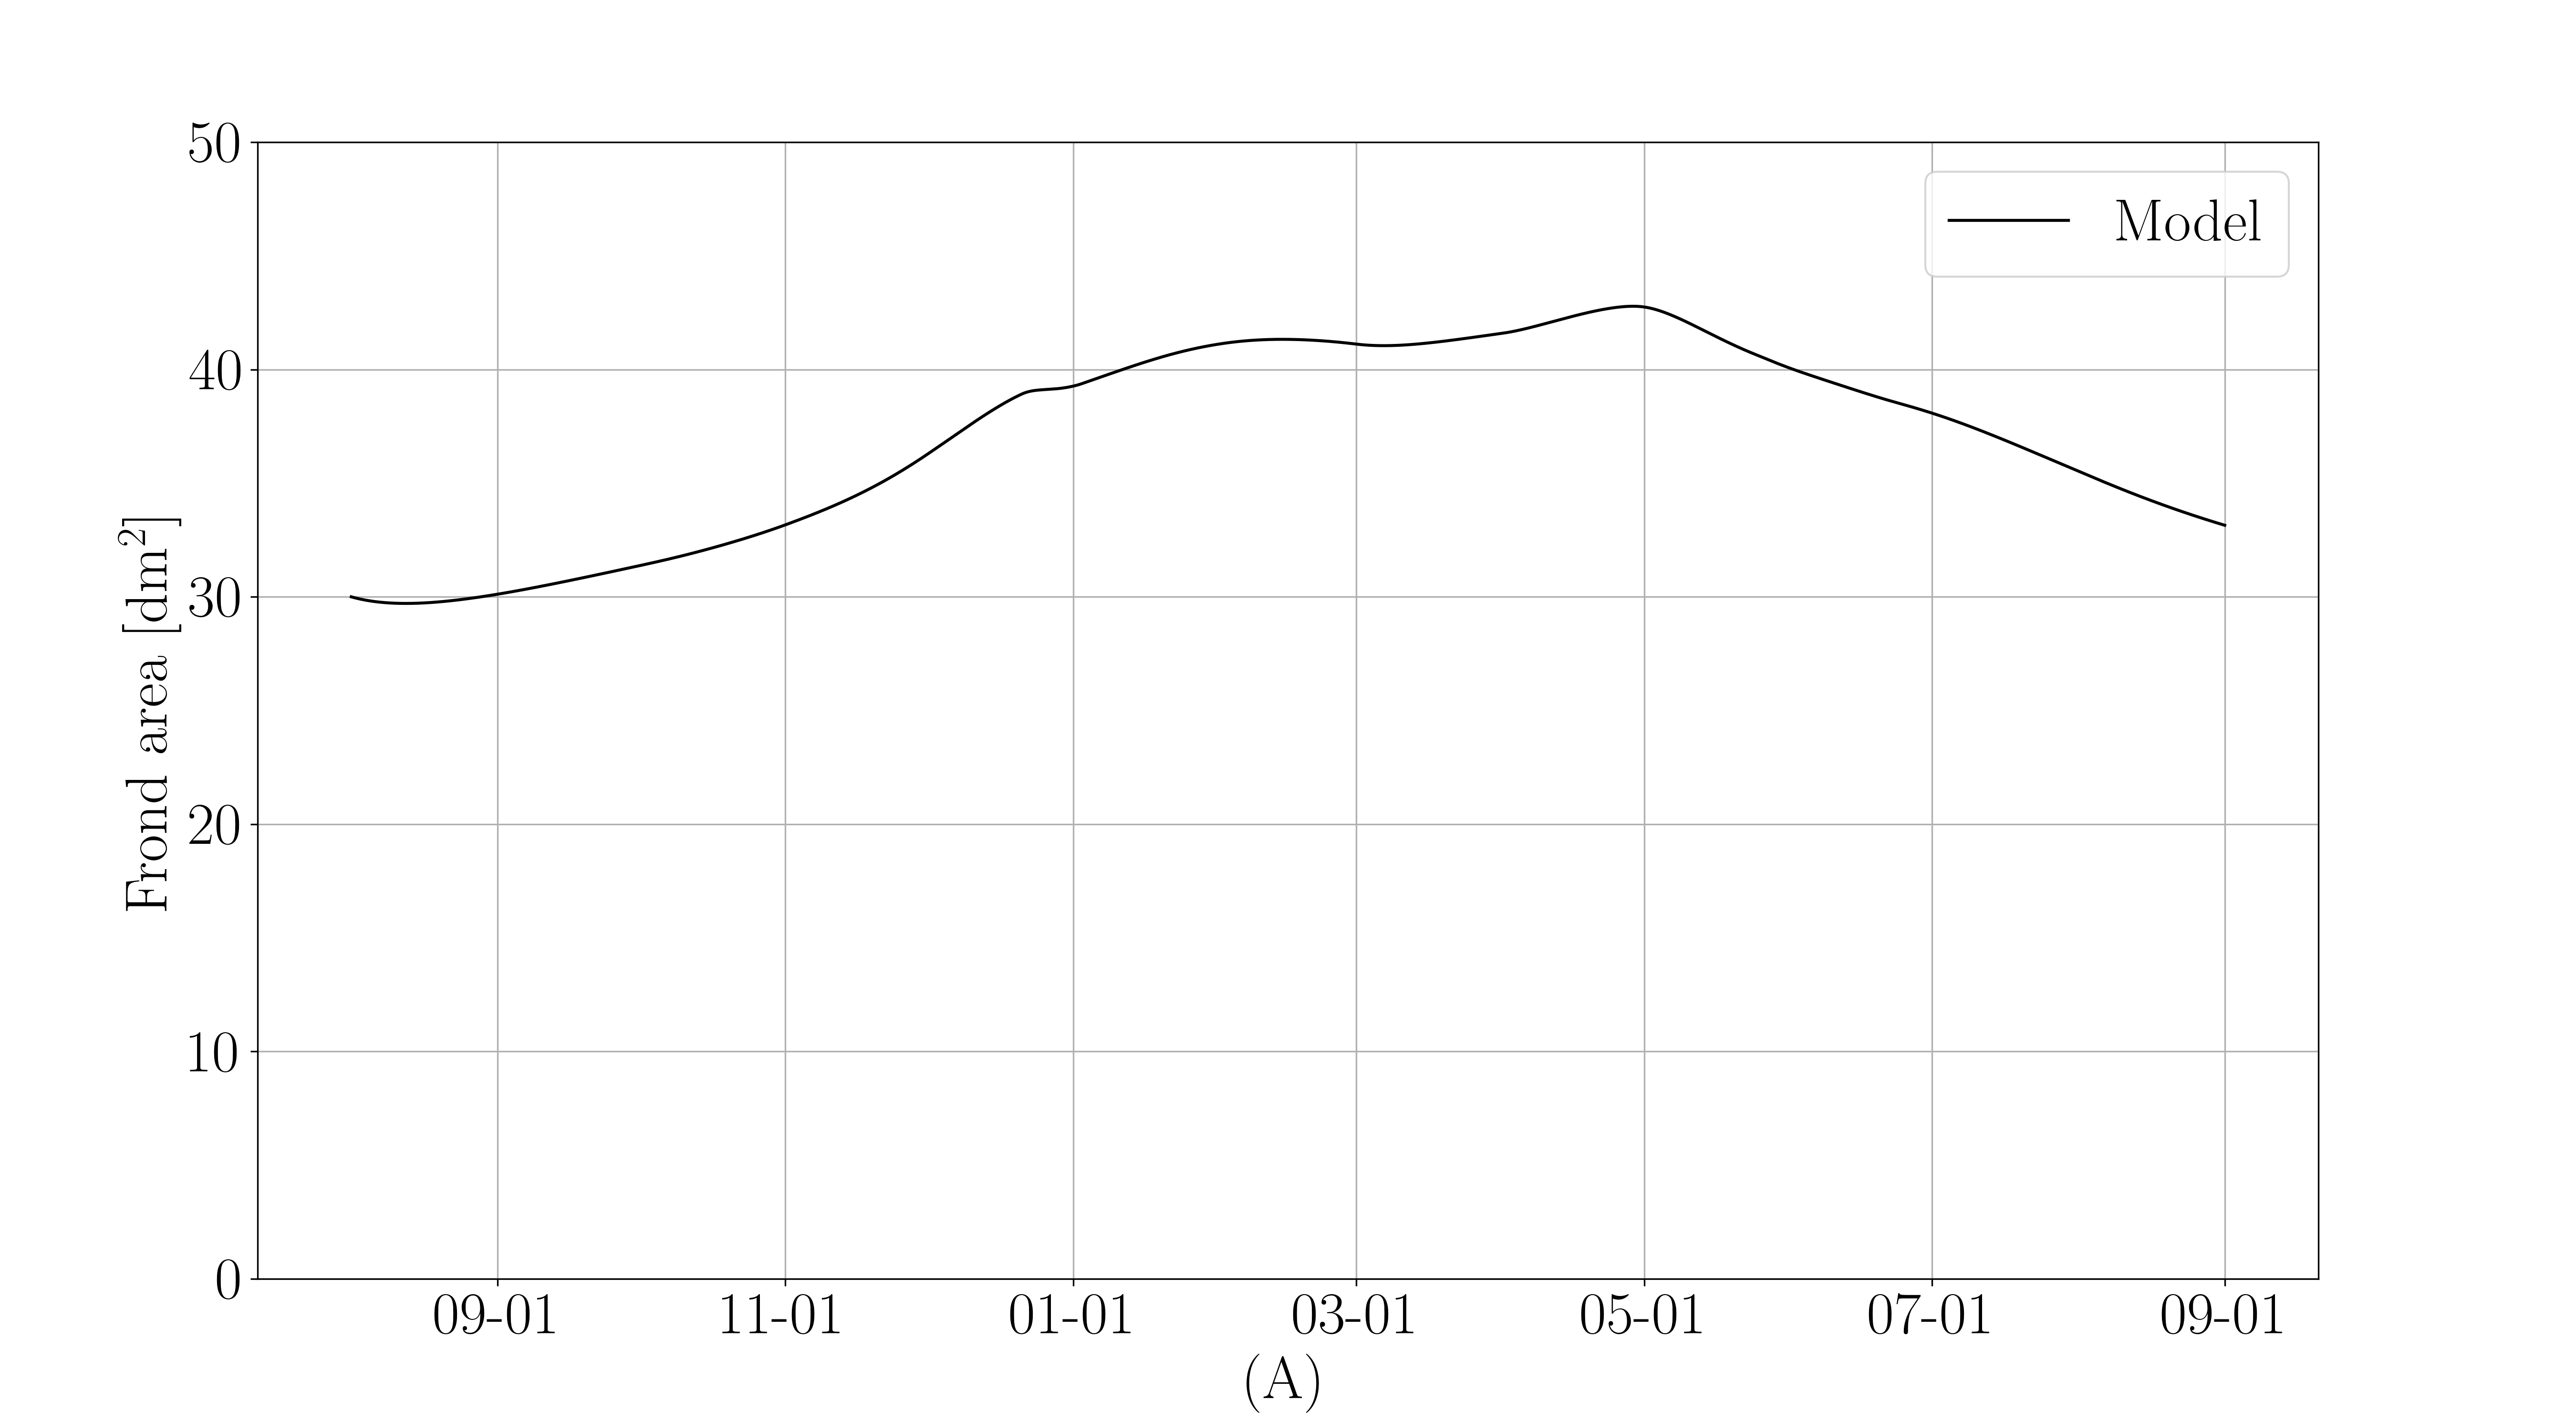
\includegraphics[width=1\linewidth]{figures/frond_area}
	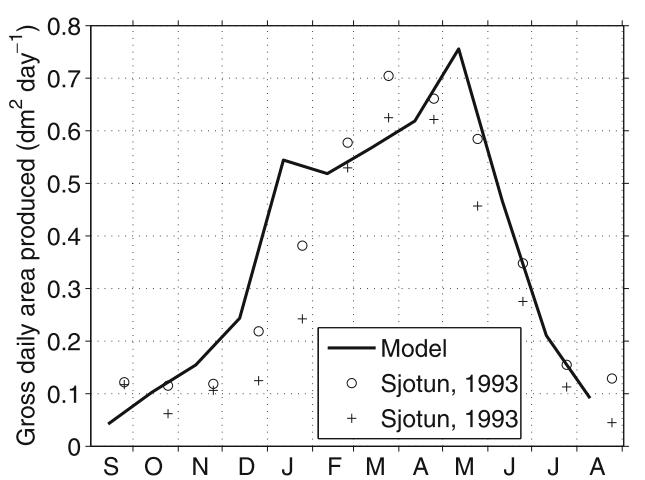
\includegraphics[width=1\linewidth]{figures/production}
	\caption{\textbf{(A)} Standing frond area. \textbf{(B)} Gross daily frond area produced. \textit{Solid line}, model results. \textit{Circles}, daily area produced estimated from Sjotun (1993), 2-year plants. \textit{Crosses}, daily area produced estimated from\cite{sjotun1993}, 3-year plants}
	\label{fig:biomass}
\end{figure}

\begin{figure}[H]
	\centering
	\includegraphics[width=1\linewidth]{figures/carbon_storage}
	\includegraphics[width=1\linewidth]{figures/nitrogen_storage}
	\caption{\textbf{(A)} Carbon content expressed as a fraction of dry weight. \textit{Solid line}, model results. \textit{Circles}, \cite{sjotun1993} proximal/meristematic tissue. \textit{Crosses}, apical frond tissue. \textbf{(B)} Nitrogen content expressed as fraction dry weight. \textit{Solid line}, model results. \textit{Circles}, \cite{sjotun1993} 2-year plants. \textit{Crosses}, \cite{sjotun1993}, 3-year plants.}
	\label{fig:storage}
\end{figure}

\section{Testcase: Tidal flume farm}
The tidal flume farm test case is a synthetic case used to test the 3D performance of the model in Delft3D flexible mesh with sigma layers. It is designed to demonstrate that the biomass allocation works with variable sigma layer thickness in time due to tidal variation.

The test case consists of a 10x30 cell grid with 100 m resolution containing a factor 2 refinement  in the center to obtain a 50m resolution. The model is thus 1km x 3km. It has a uniform depth of 10 m and 20 sigma layers, meaning each layer is 0.5 m deep. The tidal amplitude applied is 2 m and velocities vary between 0.0-0.1 m/s. The flow switches direction approximately every 6 hours. The oscillation of the layer thickness means each layer will be between 0.4 m (low water) and 0.6 m (high water) thick. Thus as long as the plant is at least 0.4 m long and grows a minimum of 0.4 m, the segments within which it resides will vary within a single tidal period due to water level variations alone. Multiple farms are located within this higher resolution area. The layout is shown in Figure \ref{fig:tidalflumefarm}

\begin{figure}[H]
	\centering
	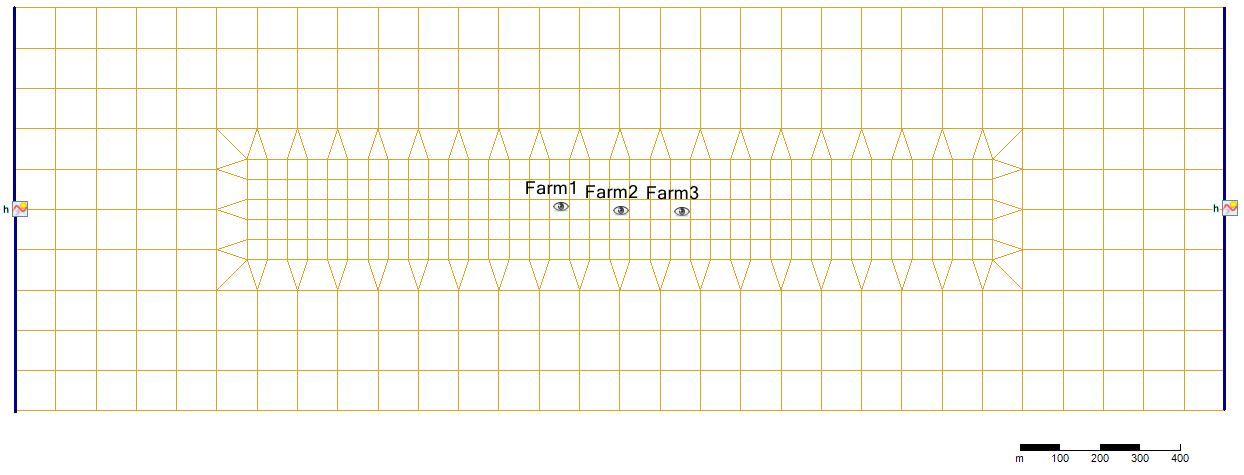
\includegraphics[width=1\linewidth]{figures/tidal_flume_farm}
	\caption{Layout of the tidal flume farm test case}
	\label{fig:tidalflumefarm}
\end{figure}

This model was run with 4 different settings:
\begin{itemize}
	\item Put 903g in a 2500 m$^{2}$ cell, equivalent to 0.159 gC m$^{-2}$ biomass in single cell, no length correction
	\item increase biomass 100x
	\item stretch standard amount of biomass to 7m in length
	\item stretch 100x biomass to 7m in length
\end{itemize}

These models were used to test the implementation of various features of the code.

\chapter{References}
\bibliography{MALG_manual}

\end{document}